\documentclass[12pt,]{article}
\usepackage{lmodern}
\usepackage{amssymb,amsmath}
\usepackage{ifxetex,ifluatex}
\usepackage{fixltx2e} % provides \textsubscript
\ifnum 0\ifxetex 1\fi\ifluatex 1\fi=0 % if pdftex
  \usepackage[T1]{fontenc}
  \usepackage[utf8]{inputenc}
\else % if luatex or xelatex
  \ifxetex
    \usepackage{mathspec}
  \else
    \usepackage{fontspec}
  \fi
  \defaultfontfeatures{Ligatures=TeX,Scale=MatchLowercase}
    \setmainfont[]{Times New Roman}
\fi
% use upquote if available, for straight quotes in verbatim environments
\IfFileExists{upquote.sty}{\usepackage{upquote}}{}
% use microtype if available
\IfFileExists{microtype.sty}{%
\usepackage{microtype}
\UseMicrotypeSet[protrusion]{basicmath} % disable protrusion for tt fonts
}{}
\usepackage[margin=2.54cm]{geometry}
\usepackage{hyperref}
\hypersetup{unicode=true,
            pdftitle={Examining the Hydrologic Properties of the Missouri River Basin},
            pdfauthor={Rachel Bash, Keqi He, Caroline Watson, and Haoyu Zhang},
            pdfborder={0 0 0},
            breaklinks=true}
\urlstyle{same}  % don't use monospace font for urls
\usepackage{longtable,booktabs}
\usepackage{graphicx,grffile}
\makeatletter
\def\maxwidth{\ifdim\Gin@nat@width>\linewidth\linewidth\else\Gin@nat@width\fi}
\def\maxheight{\ifdim\Gin@nat@height>\textheight\textheight\else\Gin@nat@height\fi}
\makeatother
% Scale images if necessary, so that they will not overflow the page
% margins by default, and it is still possible to overwrite the defaults
% using explicit options in \includegraphics[width, height, ...]{}
\setkeys{Gin}{width=\maxwidth,height=\maxheight,keepaspectratio}
\IfFileExists{parskip.sty}{%
\usepackage{parskip}
}{% else
\setlength{\parindent}{0pt}
\setlength{\parskip}{6pt plus 2pt minus 1pt}
}
\setlength{\emergencystretch}{3em}  % prevent overfull lines
\providecommand{\tightlist}{%
  \setlength{\itemsep}{0pt}\setlength{\parskip}{0pt}}
\setcounter{secnumdepth}{5}
% Redefines (sub)paragraphs to behave more like sections
\ifx\paragraph\undefined\else
\let\oldparagraph\paragraph
\renewcommand{\paragraph}[1]{\oldparagraph{#1}\mbox{}}
\fi
\ifx\subparagraph\undefined\else
\let\oldsubparagraph\subparagraph
\renewcommand{\subparagraph}[1]{\oldsubparagraph{#1}\mbox{}}
\fi

%%% Use protect on footnotes to avoid problems with footnotes in titles
\let\rmarkdownfootnote\footnote%
\def\footnote{\protect\rmarkdownfootnote}

%%% Change title format to be more compact
\usepackage{titling}

% Create subtitle command for use in maketitle
\providecommand{\subtitle}[1]{
  \posttitle{
    \begin{center}\large#1\end{center}
    }
}

\setlength{\droptitle}{-2em}

  \title{Examining the Hydrologic Properties of the Missouri River Basin}
    \pretitle{\vspace{\droptitle}\centering\huge}
  \posttitle{\par}
  \subtitle{\url{https://github.com/cwatson1013/Hydrologic_Data_Analysis_Final_Proj}}
  \author{Rachel Bash, Keqi He, Caroline Watson, and Haoyu Zhang}
    \preauthor{\centering\large\emph}
  \postauthor{\par}
    \date{}
    \predate{}\postdate{}
  
\usepackage{booktabs}
\usepackage{longtable}
\usepackage{array}
\usepackage{multirow}
\usepackage{wrapfig}
\usepackage{float}
\usepackage{colortbl}
\usepackage{pdflscape}
\usepackage{tabu}
\usepackage{threeparttable}
\usepackage{threeparttablex}
\usepackage[normalem]{ulem}
\usepackage{makecell}
\usepackage{xcolor}

\begin{document}
\maketitle
\begin{abstract}
The Missouri River provides critical water resources that drives the
region's agriculture, industry, and ecosystems. This is a region that
experiences surface water variability, characterized by damaging floods
and severe droughts, greatly impacting the agricultural production of
the area. It is reported that a serious flood disaster occurred in the
lower Missouri River in the spring of 2019 and the Missouri River
experienced severe drought in 2012-2013. This project highlights the
changes in stream flow and water quality over time, and identifies key
characteristics of the river. Twenty two sites across the lower Missouri
River Basin were examined in order to get a fuller picture of the
Missouri River and its tributaries over time. By analyzing the trend of
the Missouri River discharge, we can predict future changes in the
Missouri River flow to provide a reference for water resources
management. In addition, we focus on the stream flow and water quality
of Missouri River during March to July, 2019 to see how discharge
influence the water quality and what can be done to keep the water in
the Missouri River in good quality.
\end{abstract}

\newpage
\tableofcontents 
\newpage
\listoftables 
\newpage
\listoffigures 
\newpage

\hypertarget{research-question-and-rationale}{%
\section{Research Question and
Rationale}\label{research-question-and-rationale}}

The Missouri River is the largest river in North America (2,540 miles)
and has the second largest watershed (529,000 mi\textsuperscript{2}/339
acres, U.S.-Canada). Its watershed covers portions of ten states, which
account for approximately one-sixth of the continental United States, as
well as a small part of Canada. The headwater is located in the
Bitterroot Mountains River of northwestern Wyoming and southwestern
Montana. The watershed is home to around 12 million people in 1990, and
has been inhabited by indigenous people for millennia. Demands for
managing the river for the benefit of human livelihood has resulted in
drastic modification in the river and the floodplains. Numerous
reservoirs and dams have been constructed, of which six major dams were
built on the mainstream, following the Pick-Sloan Plan in 1944. Now, the
river is used intensively in multiple ways, including municipal,
agricultural, hydropower, recreation, flood control etc.

Within the 328 million acres of the basin's total area in the United
States, 95\% is related to agricultural uses, while the rest dedicated
for recreation, fish and wildlife, and urban. More than half of the
total is pasture and range grassland primarily for grazing, and cropland
consists of almost 104 million acres, which is 32\% of the whole basin.
Irrigated land comprises 7.4 million acres, and 6.9 million acres are
intensively cropped. Water bodies, on the other hand, cover 3.9 million
acres. In spite of the low proportion of water areas (1.2\%), they are
the pivotal foundation for agricultural or other usages, and thus
critical to the whole region's economy.

Along with the agricultural, urban, and industrial development in the
region is nutrient loading and enrichment in water bodies, especially
for nitrogen (N) and phosphorus (P). Unlike other regions, agricultural
input through fertilizer is the predominant anthropogenic source for
nutrient in water bodies in the whole basin. Regardless of the major
anthropogenic source, nutrient enrichment is considered nationally as
one of the leading factors for water quality impairment. According to
USEPA 303(d) lists, more than 160 stream reaches, lakes, or reservoirs
were reported by USEPA to suffer nutrient-related impairment in 2006.

In addition to change in nutrient concentration, discharge appears to be
highly variable in the basin, and both severe drought and flooding
events occurred in the basin in the past. For example, in the spring and
summer of 2011, an unprecedented flooding event caused over \$2 billion
damage FEMA disaster declaration was made in all states along the
Missouri River. Subsequently, in 2012, a drought even struck the Central
Great Plain, including the basin, and inflicted at least \$12 billion of
loss before July, 2012. Recently, another flooding event occurred in the
spring of 2019.

Given all the background information above, we would like to know the
current state of Missouri River and its tributaries, with a focus on the
changing pattern in discharge and nutrient. Since regions along the
downstream are more likely to be impaired by nutrient loaded and
accumulating upstream, in this project study sites were concentrated in
the southeast of the whole basin (\autoref{fig:sitemap}). We are
interested in how the dramatic change in discharge (i.e.~water quantity)
could potentially interact with nutrient enrichment (i.e.~water
quality). Also, we examined a few specific flooding events, during which
changes in both water quality and quantity were well recorded, so that
we could make concrete inference on the interplay between quantity and
quality. Finally, based on the pattern in the past and the best model we
could fit, we attempted to predict the likely future conditions and
trends in the Missouri River Basin.

\textless\textless\textless\textless\textless\textless\textless{} HEAD
Given the interesting hydrologic history of this region, we are
interested in the past, present, and future conditions of the Missouri
River and its tributaries. Our research questions and acccompanying
hypotheses are below:

1.How have changes in discharge (i.e.~water quantity) interacted with
nutrient enrichment (i.e.~water quality) in the Missouri River Basin?

\begin{verbatim}
a) Nutrient levels have increased over time
b) Discharge has become more variable over time
\end{verbatim}

\begin{enumerate}
\def\labelenumi{\arabic{enumi}.}
\setcounter{enumi}{1}
\item
  What effects do specific flood and drought events have on the water
  quality and quantity of rivers in the Missouri River Basin areas of
  interest?

  \begin{enumerate}
  \def\labelenumii{\alph{enumii})}
  \tightlist
  \item
    Rivers will exhibit a flushing behavior due to the land use and type
    of flow during storms
  \item
    Discharge will decrease during drought, causing nutrient levels to
    also decrease due to decreased overland flow.
  \end{enumerate}
\item
  Given past and current data, what can we predict about the future
  state of water in the Missouri River Basin?

  \begin{enumerate}
  \def\labelenumii{\alph{enumii})}
  \tightlist
  \item
    Total flow in the Missouri River Basin is decreasing
    (non-stationary) over time
  \item
    The future situation of the river basin will see the continuation of
    current trends of decreasing overall volume of flow.
  \end{enumerate}
\end{enumerate}

=======

\begin{figure}
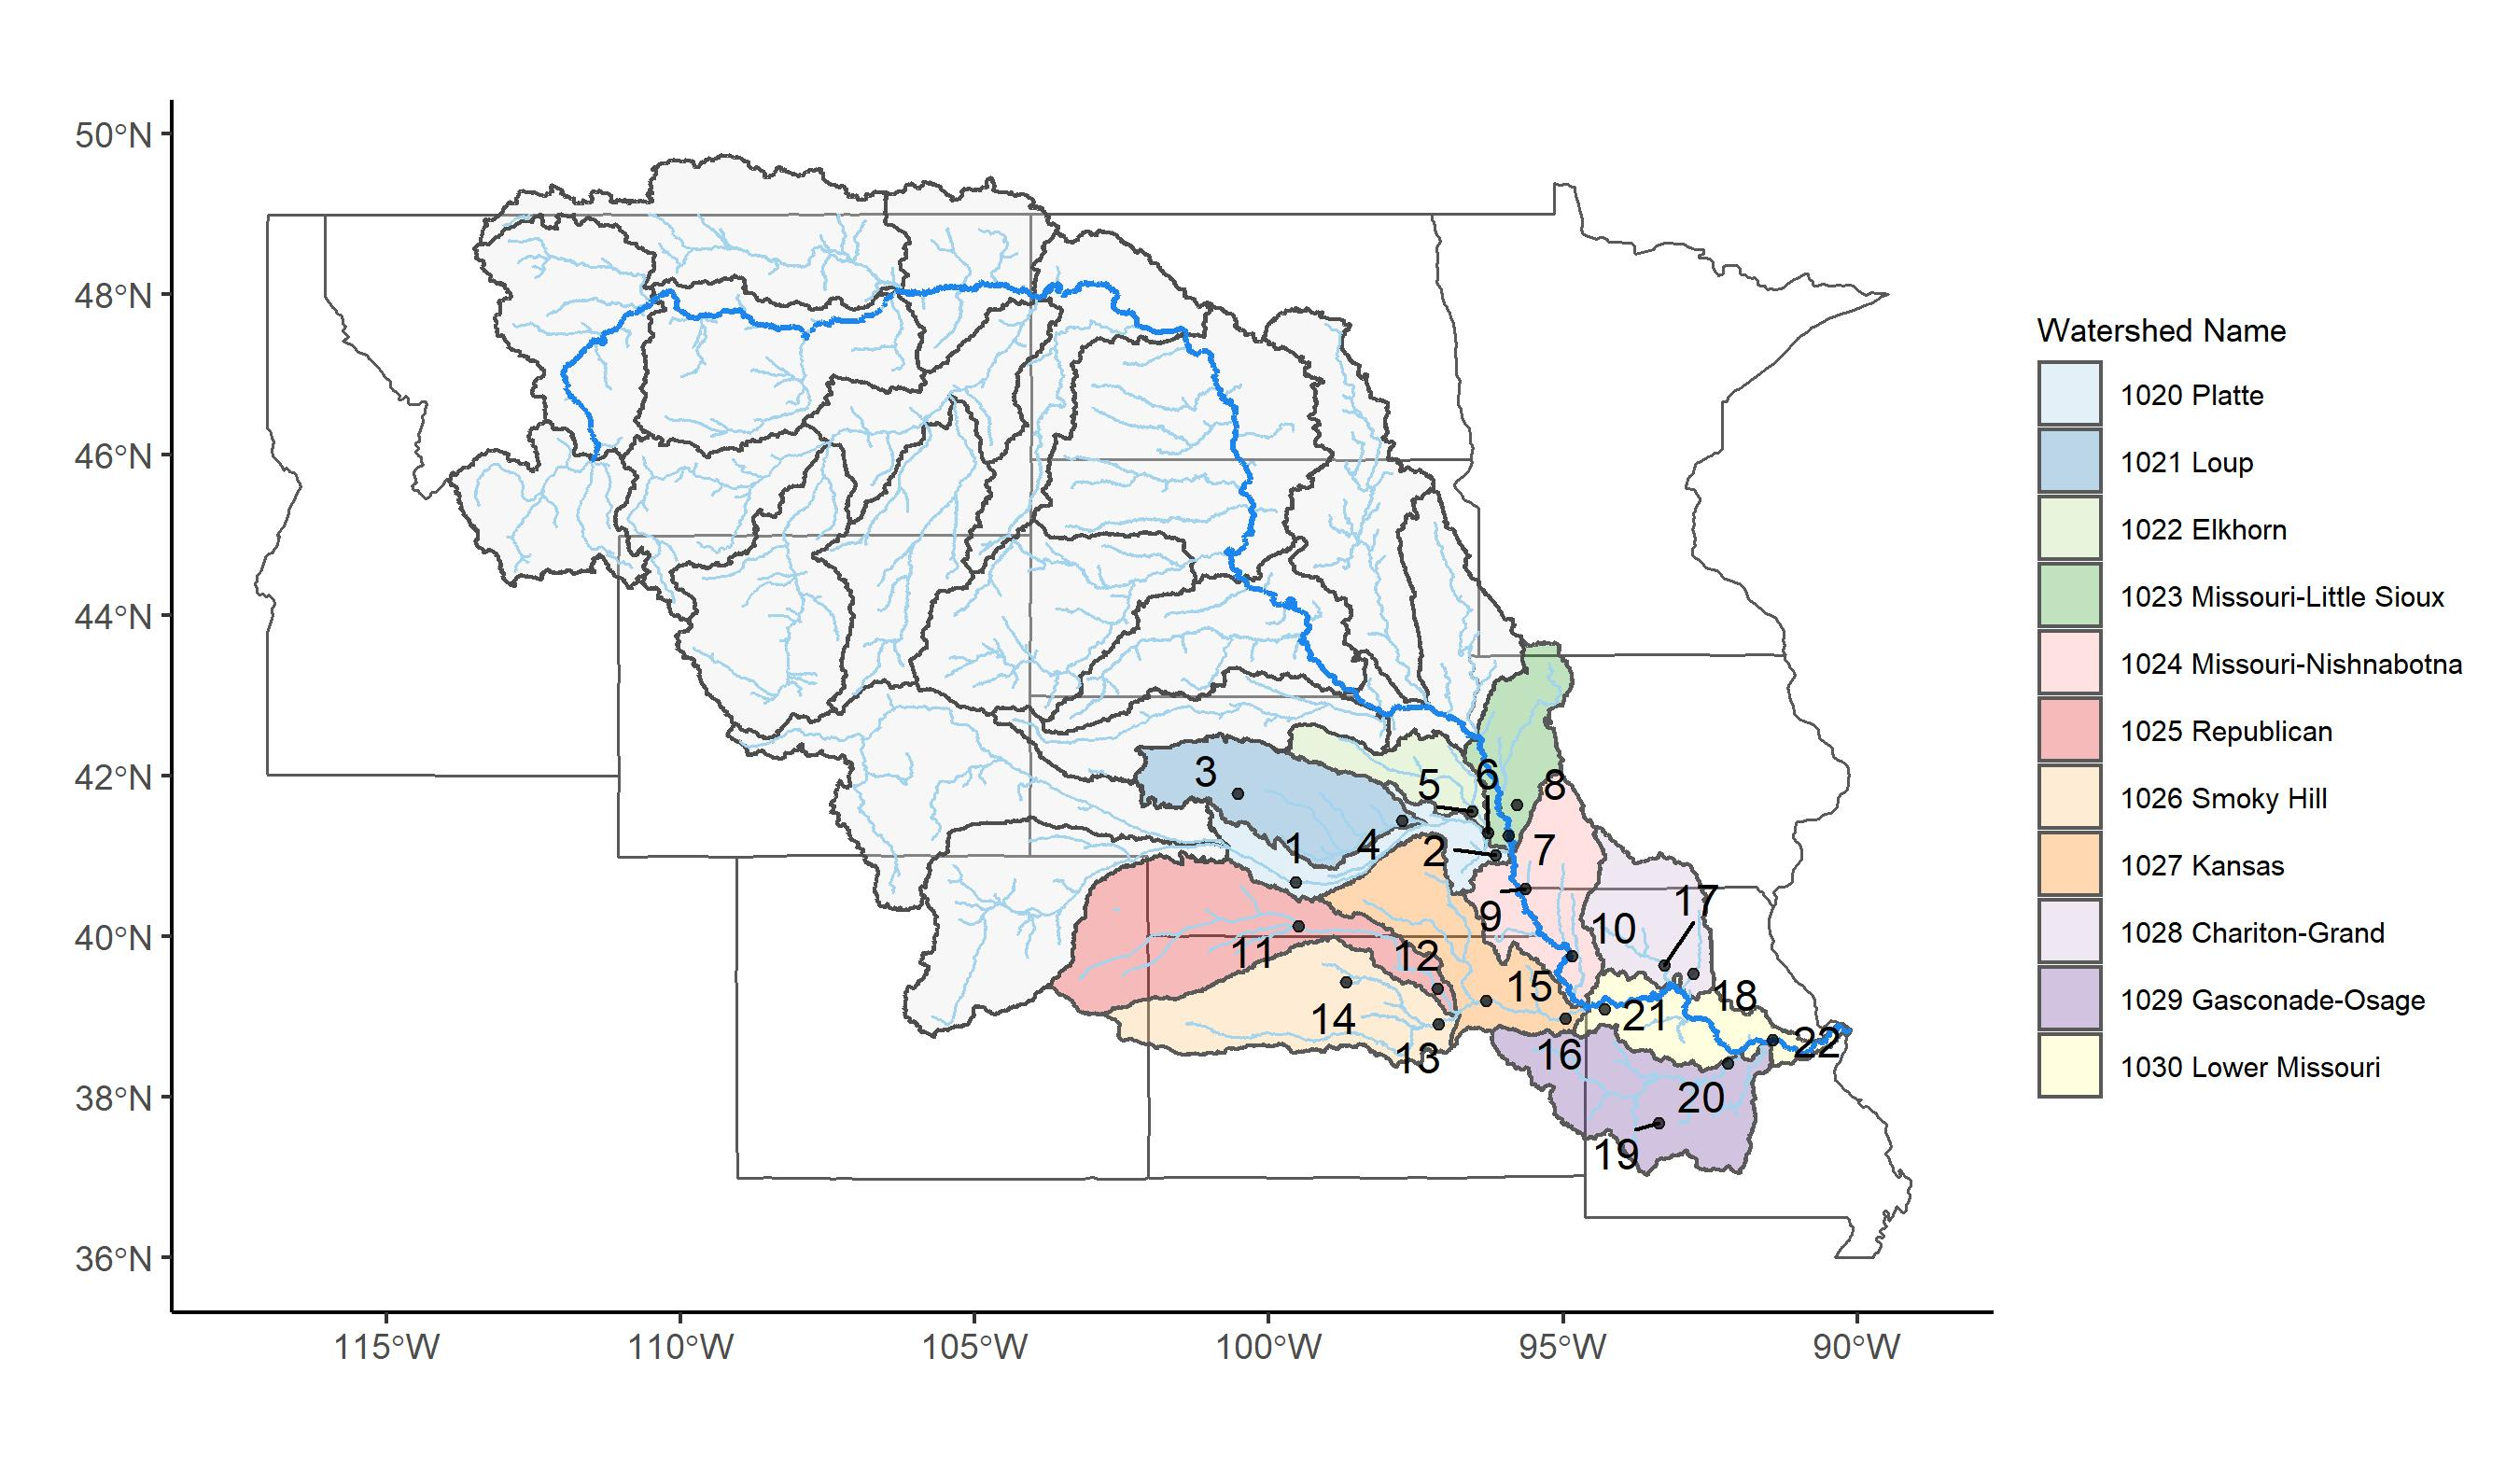
\includegraphics[width=\maxwidth]{../../Figures/site_map} \caption{\label{fig:sitemap} Map of USGS sites used for long term analysis.}\label{fig:sitemap}
\end{figure}

\newpage

\hypertarget{dataset-information}{%
\section{Dataset Information}\label{dataset-information}}

The data we are analyzing comes from the United States Geological Survey
(USGS) database called the National Water Information System interface,
or NWIS. We pulled data from the interface using the R package
\texttt{dataRetrieval}. Because we are interested in the lower Missouri
River basin, we pulled sites from each HUC4 subbasin from 1020 to 1030
(see Figure below). We chose these subbasins because they had a variety
of tributaries that all flowed into the Missouri River, representing a
variety of river sizes and lengths. We filtered these subbasin queries
to only show us sites that had discharge, nitrogen, and phosphorus data.
Once we found the sites with all of this data, we chose 2 sites from
each HUC sub basin as our 22 ``best sites''. Our best sites had the
overall best time period range for all of our ``must have'' variables.
We retrieved data on water quantity, water quality (N, P
concentrations), pH, and coliform concentrations. @ref\{tab:table\}
illustrates the variables we examined and the number of sites in our
area of interest that had quality data for each.

Only seven sites within our HUC subbasin boundary contained any high
frequency discharge and nitrogen data. Therefore, we also looked at
these 7 sites in order to do analyses and answer our research question
about flooding.

After doing initial data wrangling and analysis on our 22 ``best
sites'', we decided to pare it down further and only do subsequent
analyses on \textbf{10} sites. While we initially wanted to look at many
sites that were varied in size and location, we determined that it was
too many to look at and draw relevant conclusions from.

We have three main datasets:

\begin{itemize}
\item
  The daily values dataset with our 22 ``best sites''
\item
  The water quality dataset with our 22 ``best sites'', with only six
  sites that had total coliform data.
\item
  The high freqency dataset with 7 sites that contain both high
  frequency discharge and high frequency nitrogen data.
\end{itemize}

\begin{table}[H]
\centering
\begin{tabular}{l|l|l}
\hline
Variables & Units & NumOfSites\\
\hline
discharge & cfs or m3/s & 22\\
\hline
time & UTC & 22\\
\hline
nitrogen & mg/L & 22 daily values, 7 high frequency\\
\hline
pH & 1 & 22\\
\hline
total coliform & cfu/100mL & 6\\
\hline
phosphorus & mg/L & 22\\
\hline
\end{tabular}
\end{table}

\newpage

\hypertarget{exploratory-data-analysis-and-wrangling}{%
\section{Exploratory Data Analysis and
Wrangling}\label{exploratory-data-analysis-and-wrangling}}

\hypertarget{yearly-discharge-pattern}{%
\subsection{Yearly Discharge Pattern}\label{yearly-discharge-pattern}}

Typical discharge patterns within a year for each HUC4 watershed from
1020 to 1030 were generated by compiling all available discharge data at
each USGS site, and two sites in the same HUC4 watershed were plotted in
the same panel with different colors (\autoref{fig:dispattern}).
Generally, discharge reaches its peak during the summer and falls to
minima during the winter. Most of basins exhibit rather high variations
across years, as indicated the large difference between the medians and
maxima or minima. Furthermore, highest variations in discharge appear to
occur in the summer, whereas discharge in the winter varies less across
years.

\begin{figure}
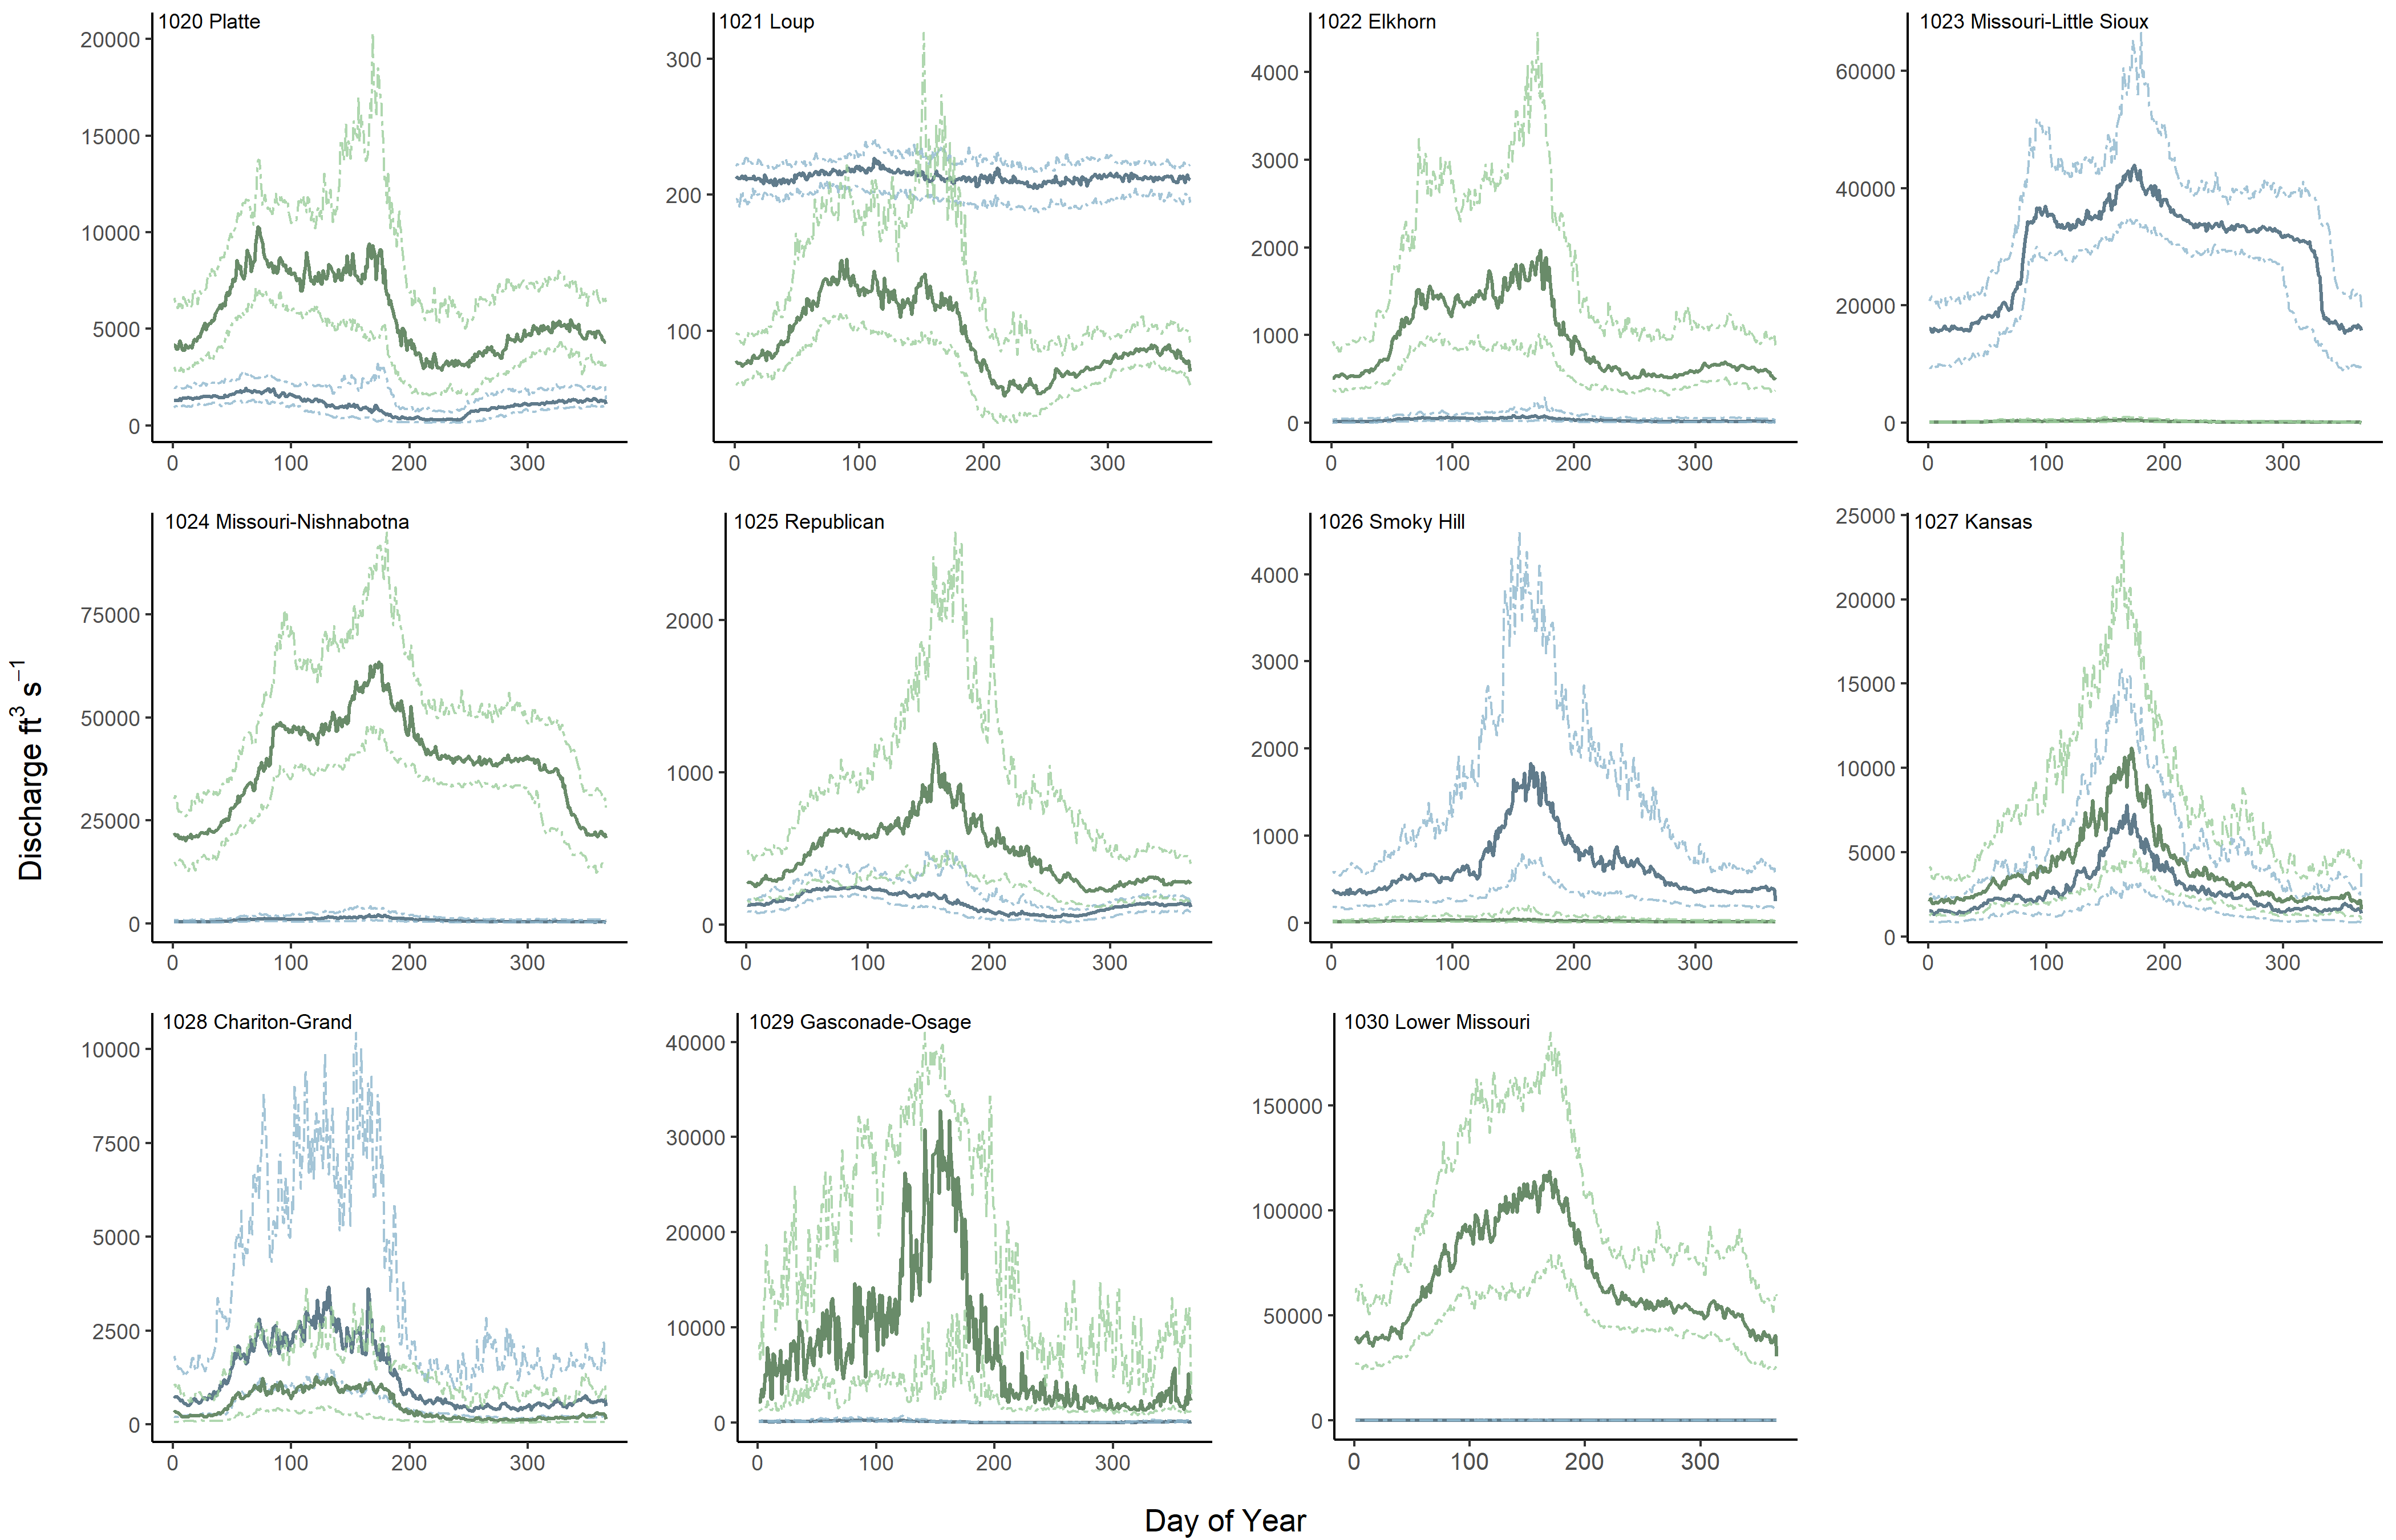
\includegraphics[width=\maxwidth]{../../Figures/discharge} \caption{\label{fig:dispattern}Yearly discharge pattern for 11 HUC4 watersheds. Thick, dark lines are the median of all discharge records on a day of year, while light, thin lines are the maximum and minimum discharge on that day.}\label{fig:dispattern}
\end{figure}

\begin{longtable}[]{@{}rcccc@{}}
\caption{Slopes of linear regression between year and standard deviation
of discharge at 22 sites.}\tabularnewline
\toprule
~ & Site Name & HUC4 & \(\beta_1\) & \emph{P}\tabularnewline
\midrule
\endfirsthead
\toprule
~ & Site Name & HUC4 & \(\beta_1\) & \emph{P}\tabularnewline
\midrule
\endhead
1 & Platte River near Overton, Nebr. & 1020 & -0.805 &
0.83\tabularnewline
2 & Platte River at Louisville, Nebr. & 1020 & 33.6 &
0.145\tabularnewline
3 & Dismal River near Thedford, Nebr. & 1021 & 0.047 &
0.196\tabularnewline
4 & Beaver Creek at Genoa, Nebr. & 1021 & 0.168 & 0.812\tabularnewline
5 & Maple Creek near Nickerson, Nebr. & 1022 & 1.1 &
0.314\tabularnewline
\textbf{6} & \textbf{Elkhorn River at Waterloo, Nebr.} & \textbf{1022} &
\textbf{11.7} & \textbf{0.009}\tabularnewline
\textbf{7} & \textbf{Missouri River at Omaha, NE} & \textbf{1023} &
\textbf{-95.2} & \textbf{0.0093}\tabularnewline
8 & Boyer River at Logan, IA & 1023 & 2.4 & 0.134\tabularnewline
\textbf{9} & \textbf{Nishnabotna River above Hamburg, IA} &
\textbf{1024} & \textbf{13} & \textbf{0.0018}\tabularnewline
10 & Missouri River at St.~Joseph, MO & 1024 & -32.1 &
0.452\tabularnewline
\textbf{11} & \textbf{Republican River near Orleans, Nebr.} &
\textbf{1025} & \textbf{-5.86} & \textbf{1e-04}\tabularnewline
12 & REPUBLICAN R AT CLAY CENTER, KS & 1025 & -5.58 &
0.157\tabularnewline
13 & SMOKY HILL R AT ENTERPRISE, KS & 1026 & -12.9 &
0.226\tabularnewline
14 & SF SOLOMON R AT OSBORNE, KS & 1026 & -5.27 & 0.0716\tabularnewline
15 & KANSAS R AT WAMEGO, KS & 1027 & -6.68 & 0.714\tabularnewline
16 & KANSAS R AT DESOTO, KS & 1027 & 2.56 & 0.91\tabularnewline
\textbf{17} & \textbf{Grand River near Sumner, MO} & \textbf{1028} &
\textbf{40.4} & \textbf{0.0264}\tabularnewline
\textbf{18} & \textbf{Chariton River near Prairie Hill, MO} &
\textbf{1028} & \textbf{11.9} & \textbf{0.0199}\tabularnewline
19 & Pomme de Terre River near Polk, MO & 1029 & 1.39 &
0.704\tabularnewline
20 & Osage River below St.~Thomas, MO & 1029 & 138 &
0.311\tabularnewline
21 & Little Blue River near Lake City, MO & 1030 & 2.1 &
0.141\tabularnewline
22 & Missouri River at Hermann, MO & 1030 & 0.657 & 0.994\tabularnewline
\bottomrule
\end{longtable}


\end{document}
